
\subsubsection{Dichtungsrahmen}
Die Flachstangen wurden zusammengeschweißt und mit einem Tiefschwarz Lackspray lackiert. Der Rahmen wird aus 4mm dickem und 35mm breiten Flachstangen erstellt. Auf diesen Rahmen kommt ein Dichtungsband und die Tür wird dann mit sogenannten Kniehebelspanner an den Rahmen gedrückt. So ist es möglich, die Kammer Luft und Staubdicht zu verschließen. Der Rahmen wird an den Seiten an das Gestell geklebt und unten sowie oben in eine Nut eingelassen.
\vspace{5mm}
\begin{table}[H]
    \centering
    \begin{tabular}{ | c | c | } 
  \hline
   \textbf{Bezeichnung} & \textbf{Stückzahl}\\ 
  \hline
   Flachstange 35x580mm & 2\\ 
  \hline
   Flachstange 20x664mm & 1 \\ 
  \hline
  Flachstange 35x664mm & 1 \\ 
  \hline
  Schaumisolierung 3m & 1 \\ 
  \hline
\end{tabular}
    \caption{Stückliste Dichtungsrahmen}
\end{table}
\vspace{5mm}
\begin{figure}[H]
    \centering
    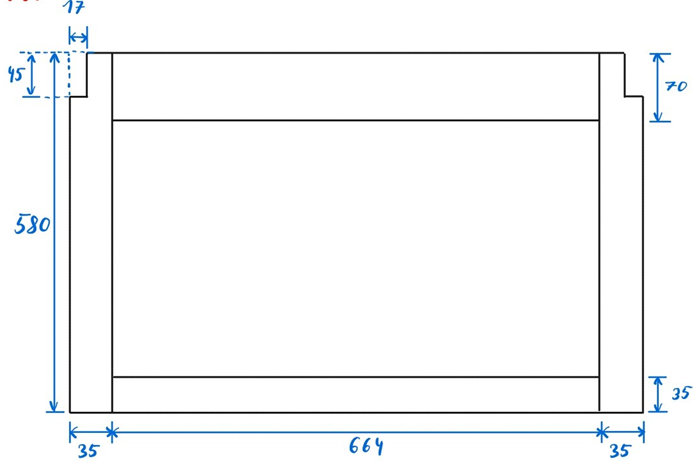
\includegraphics[scale=1.2]{image/skizzerahmen.png}
    \caption{Skizze Dichtungsrahmen in mm}
    \label{fig:enter-label}
\end{figure}
Die Flachstangen werden zusammengeschweißt und dann mit einem Tiefschwarz Lackspray lackiert. Das Dichtungsband wird doppelt mit einem Abstand dazwischen auf den Rahmen geklebt. \\
Das Schaumisolierbar hat eine hervorragende Dicht- und Verformungsbeständigkeit, ist für Temperaturen von -50°C bis 150°C geeignet, hat eine gute Dämpfung sowie eine gute \\
Wärmeisolierung.
\begin{figure}[H]
    \centering
    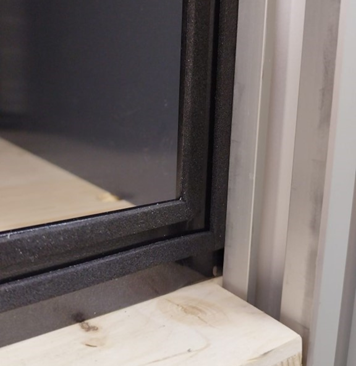
\includegraphics{image/rahmen2.png}
    \caption{Rahmen}
    \label{fig:enter-label}
\end{figure}
\vspace{5mm}
